\documentclass[a4paper,12pt]{article}
\usepackage[latin1]{inputenc}
\usepackage[spanish]{babel}
\usepackage{graphicx}
\usepackage{amsmath}
\usepackage{wrapfig}
\setlength{\textheight}{250mm}
\setlength{\textwidth}{165mm}
\setlength{\topmargin}{-15mm}
\setlength{\oddsidemargin}{0pt}
\pagestyle{empty}

\begin{document}

\def\bm#1{{\mbox{\boldmath $#1$}}}
\def\eqdef{\buildrel \rm def \over =}
\def\signo{\mathop{\rm signo}\nolimits}

\mbox{}\vspace*{-20mm}

{\centering
{\small\sc Escuela T�cnica Superior de Ingenieros de Caminos, Canales y Puertos (Madrid)}\\*[4mm]
{\Large\bf M�todo de los Elementos Finitos }\\*[4mm]
PR�CTICA 5: Elasticidad lineal (elementos 2D). \\*[4mm]

% \vspace{4mm}

% ENUNCIADO

En esta pr�ctica se analiza un tubo de secci�n circular y longitud
indefinida, sometido a presi�n interna. Se emplea un modelo de deformaci�n
plana.
Se comprobar�n los resultados obtenidos en tensiones y desplazamientos
con la soluci�n te�rica.

\begin{wrapfigure}{r}{50mm}
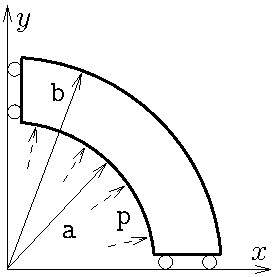
\includegraphics{cilipst}
\end{wrapfigure}

El fichero 
\texttt {Icilpst} contiene las instrucciones para generar
una malla plana para un cuarto de corona circular.  Esta geometr�a,
con las condiciones de contorno adecuadas (ver figura)
y en deformaci�n
plana, es apropiada para analizar el 
estado tensional de una secci�n cualquiera del tubo.

Las condiciones de contorno que hay que imponer vienen determinadas
por la simetr�a de la secci�n y de las cargas: a) desplazamiento
nulo en la direcci�n $y$ para todos los puntos situados en el eje $x$
y b) desplazamiento nulo en la direcci�n $x$ para los puntos del eje $y$.

Los distintos par�metros del problema se definen mediante las variables:
\begin{itemize}
\item  \texttt {a}: Radio interior del tubo;
\item \texttt {b}: Radio exterior del tubo;
\item \texttt {p}: Presi�n interna;
\item \texttt {c}: N�mero de elementos en la direcci�n circunferencial;
\item \texttt {r}: N�mero de elementos en la direcci�n radial (capas);
\end{itemize}

%\begin{wrapfigure}{r}{50mm}
%\input{prac3a.pstex_t}
%\caption{\em Modelo axilsim�trico}
%\label{fig:lad}
%\end{wrapfigure}

\noindent
{\em \underline {Nota}: en problemas de deformaci�n plana
la carga distribuida se da por unidad de longitud transversal
(direcci�n $z$)}

\paragraph{Soluci�n anal�tica.}   Las expresiones para la 
tensi�n radial $\sigma_{rr}$,
circunferencial $\sigma_{\theta \theta}$ y longitudinal $\sigma_{zz}$ 
son\footnote{ver, p. ej. Y.C. Fung, Foundations of solid mechanics. Prentice-Hall, 1965}:
\begin{equation*} 
\sigma_{rr}=-p \frac{{( b/r) }^2 -1}
{{( b/a)}^2 -1} \qquad 
\sigma_{\theta \theta}=
p \frac{{( b/r) }^2 +1}
{{( b/a)}^2 -1} \qquad 
\sigma_{zz}=\nu(\sigma_{rr}+\sigma_{\theta \theta})
=\nu p \frac{2}
{{( b/a)}^2 -1}
\end{equation*} 
Puede observarse que $\sigma_{rr}$ en la pared interior es igual
a la presi�n, mientras que en la pared exterior es nula.  Tambi�n se
observa que la tensi�n vertical es homog�nea en la secci�n.

La expresi�n general del desplazamiento radial $u_r$ es:
\begin{equation*}
u_r=\frac{(1+\nu)p}{E [{(b/a)}^2-1 ]} \left [ 
(1-2 \nu) r +\frac{b^2}{r} \right ] 
\end{equation*}
que particularizado en la pared interior ($r=a$) y en la exterior ($r=b$)
para los datos de la pr�ctica ($p=300$ MPa, $a=0.5$ m., $b=1.0$ m., 
$E=2.1 \cdot 10^5$ MPa, $\nu=0.3$) resulta:
\begin{equation*}
u_r(r=a)=1.3619 \textrm{ mm.},\qquad
u_r(r=b)=0.8667 \textrm{ mm.},\qquad
\end{equation*}
\end{document}
